\begin{abstract}
\label{sec:abstract}

\noindent {\bf Executive Summary}\\

The Transiting Exoplanet Survey Satellite (\textit{TESS}) will perform
a two-year, nearly all-sky survey for transiting exoplanets.  There do
not appear to be any fundamental obstacles to continuing science
operations for at least several years following the Primary Mission.  Any
Extended Mission will likely need to be organized while the Primary
Mission is occupying most of the \tess team's attention. 
To provide a head start to those who are planning and proposing for an
Extended Mission, this white paper presents some initial considerations.

Our recommendations are independent of the \tess Science Team, and we
stress that many factors other than prospects for planet detection will
influence the choice of an Extended Mission. We have created
an accompanying Wiki 
document\footnote{\url{https://spacebook.mit.edu/display/TESS/Extended+Missions}.
 Contact \url{luke@astro.princeton.edu}, copying \url{imeister@mit.edu}, to 
 receive an account with editing rights. The webpage includes catalogs of 
 detected planets for both the Primary and Extended Missions discussed in this 
 white paper. Read-only copies of the catalogs and the webpage are also 
 available at \textbf{URL GOES HERE}.\label{fn:wiki}} that can 
be edited by named members of the 
community to raise and discuss those broad issues.  

This report is focused narrowly on planet detection. 
Using Monte Carlo simulations, we try to anticipate the quantities and
types of planets that would be detected during several plausible
scenarios for a one-year Extended Mission following the two-year
Primary Mission. Our main focus is on strategies for scanning
the sky. For simplicity we do not compare different choices
either for the cadence of photometric measurements or for the target
stars to be selected, although different choices might prove to be
advantageous and should be studied in future work.

Throughout this report we consider six different scenarios for Year 3
of the \tess mission, illustrated in Figure~\ref{fig:strategies}:
\begin{figure*}[!tb]
	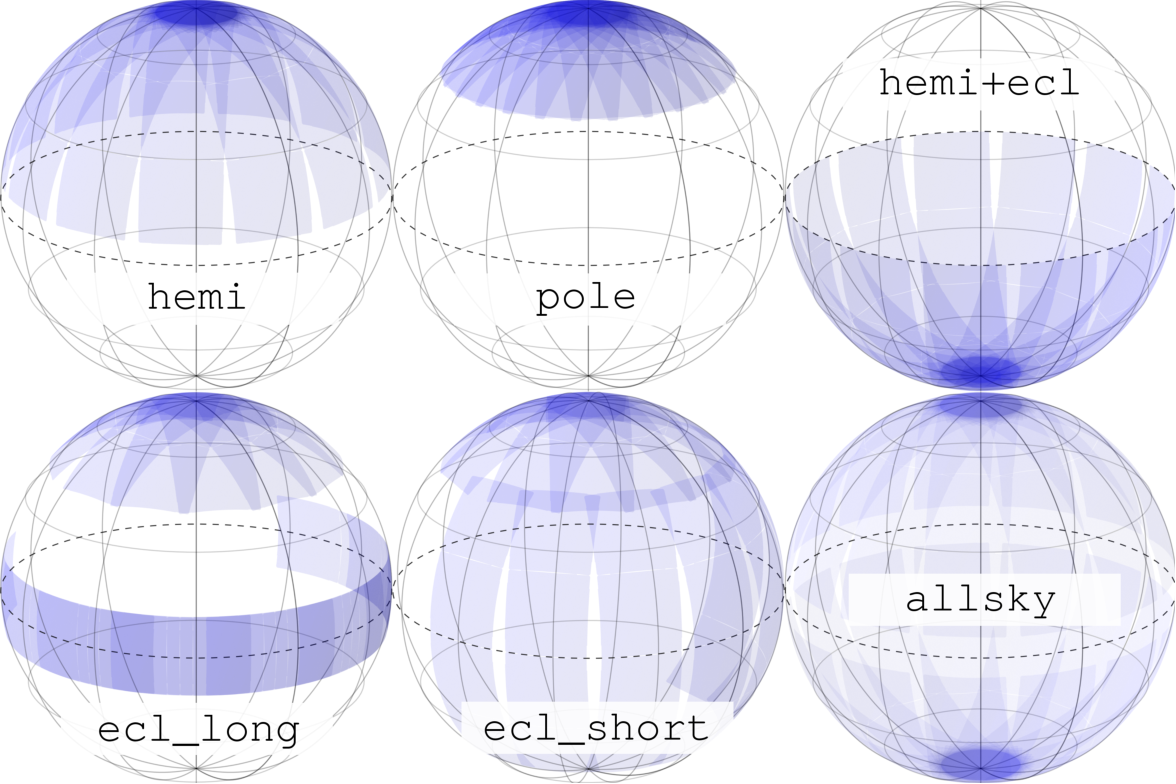
\includegraphics[width=5in]{figures/proposed_pointings_flat.pdf}
	\caption{Six proposed pointing strategies for a \tess Extended
          Mission, visualized in ecliptic coordinates.  Note that none
          of these scenarios spend the entire year observing the
          ecliptic; we concluded that such a plan would be inadvisable
          because of interruptions by the Earth and Moon (see
          Fig.~\protect\ref{fig:earth_moon_elong}).}
	\label{fig:strategies}
\end{figure*}

\begin{enumerate}

\item \nhemi, which re-observes one of the ecliptic hemispheres in
  essentially the same manner as in the Primary Mission (i.e.,
  neglecting the zone within $6^\circ$ of the ecliptic);
  
\item \npole, which focuses on one of the two ecliptic poles;
  
\item \shemiAvoid, which re-observes an ecliptic hemisphere, but moving all 
fields $6^\circ$ closer in latitude to the ecliptic plane. This scenario
has a continuous viewing zone with angular diameter $12^\circ$ rather than 
$24^\circ$;

\item \elong, which has a series of pointings with the long
  axis of the $24^\circ\times96^\circ$ field-of-view along the
  ecliptic (in combination with
  some fields near the ecliptic pole, when the Earth or Moon would
  prevent effective observations of the ecliptic);
  
\item \eshort, which has a series of pointings with the short
  axis of the field-of-view along the ecliptic (again in combination
  with some fields near the ecliptic pole);
  
\item \hemis, which covers nearly the entire sky with $\sim$14-day
  pointings (as opposed to the 28-day pointings of the Primary
  Mission), by alternating between northern and southern hemispheres.
 
\end{enumerate}

We numerically compute the results based on the methodology
of~\citet{Sullivan_2015}, after bug fixes and enhancements by Luke Bouma in
consultation with Josh Winn. Additional inputs were provided by Jacobi
Kosiarek and Peter McCullough.

Some of the most important findings are:
\begin{enumerate}

\item The overall quantity of detected planets\footnote{We define `detected 
planet' to mean one with at least two observed transits, and a phase-folded 
$\mathrm{SNR} > 7.3$ (Eq.~\ref{eq:detection_criterion}). All statistics are 
quoted for $R_p<4R_\oplus$ planets.} does not depend
  strongly on the sky-scanning schedule.  Among the six scenarios
  considered here, the number of newly-detected planets with radii
  less than $4R_\oplus$ is the same to within about 30\%.

\item The number of newly-detected sub-Neptune radius planets ($R_p \lesssim 
4R_\oplus$) in Year 3 is approximately the same as the number detected in 
either Year 1 or
  Year 2.  Thus, we do not expect a sharp fall-off in the planet
  discovery rate in Year 3.  This is because the Primary Mission will
  leave behind many short-period transiting planets with bright host
  stars, with a signal-to-noise ratio just below the threshold for
  detection.  These planets can be detected by collecting more data in
  Year 3.
      
\item Apart from detecting new planets, a potentially important
	function of an Extended Mission would be to improve our ability to
	predict the times of future transits and occultations of 
	{\it TESS}-detected planets.  With data from the Primary Mission 
	alone, the uncertainty in planetary orbital periods will inhibit 
	follow-up observations after only a few years, as the transit ephemerides
	become stale. By re-observing the same sky that was observed in the
	Primary Mission, \nhemi, \shemiAvoid, and \hemis\ address this issue.

\item Regarding newly detected sub-Neptunes, the \hemis, \npole, and
  \shemiAvoid\,strategies offer the greatest number (1350-1400, as
  compared to the 1250 during each year of the Primary Mission).
 
\item Regarding planets with orbital periods >20 days, the \hemis\:and
\npole\:strategies discover twice as many such planets as will be
discovered in each year of the Primary Mission.
However, this assumes that `detectable planets' are those with \textit{i)} at 
least two transits over both the Primary and Extended Missions, and
\textit{ii)} $\mathrm{SNR}_\mathrm{phase-folded} \geq 7.3$.
If we restrict `detections' to mean planets with $N_\mathrm{tra}\geq 3$, 
and keep the same SNR threshold, then \npole\:detects 260 new 
long-period planets, while the next-best scenarios, \hemis, \nhemi, and 
\shemiAvoid, all detect about 160. (The Primary mission detects 145; see 
Figs.~\ref{fig:yield_results} and~\ref{fig:Ntra_hist}).

\item Regarding new planets with very bright host stars ($I_c<10$),
  the \hemis, \shemiAvoid, and \eshort\:strategies offer the greatest
  numbers ($\sim\!$190, about the same as are found in each year of the
  Primary Mission; see Table~\ref{tab:icmag_meta}).

\item Regarding planets with near-terrestrial insolation ($0.2 
  <S/S_\oplus< 2$), all the strategies considered here offer similar
  numbers (about 120, as compared to 105 in each year of the Primary
  Mission).

  
  
\end{enumerate}

The rest of this report is organized as follows.
Sec.~\ref{sec:approach} discusses how we selected and compared 
different pointing strategies, 
as well as how we modeled \tesss observations and planet detections.
Sec.~\ref{sec:comparing_pointing_strategies} describe figures of merit for 
comparing any Extended Mission scenario, including those that we chose not to 
study.
Sec.~\ref{sec:input_assumptions} gives a list of the most important assumptions 
we made for the simulations.
Sec.~\ref{sec:newly_detected_planet_metrics} compares the characteristics of 
newly-detected planets, for the 6 different scenarios under consideration.
Sec.~\ref{sec:gtr_1yr_horizon} discusses some considerations and implications for future years of the Extended Mission, beyond the one-year scenarios that were simulated
in detail.
Sec.~\ref{sec:ephemeris_times} discusses the critical issue of the uncertainty in transit ephemerides.
Sec.~\ref{sec:risks_caveats} discusses the reliability and limitations of our methodology.
Sec.~\ref{sec:conclusions} concludes and recommends avenues for further study.

\end{abstract}
